% Contenido del CursoICE_2024
\chapter{Pensar de manera funcional. Programación declarativa}
\label{ch_intro}

\IndiceCapitulo
\begin{Resumen}
   Se considera que la programación funcional está basada en el \textit{cálculo lambda},  un sistema formal desarrollado en los años 1930 para investigar la naturaleza de las funciones, de la computabilidad y su relación con la recursión. 
   
   \smallskip
   
   El objetivo de este curso es explicar las técnicas y la forma funcional de razonar en programación para mejorar la calidad del código de los programas.
\end{Resumen}

\section{Adiós a la Programación Orientada a Objetos}
\label{sec_adios_poo}
\noindent A partir de los años 90 del siglo pasado, la Programación Orientada a Objetos (POO) se convirtió en el paradigma fundamental de programación. Si no sabías programar orientado a objetos, no sabías programar. Se enseñaba de una forma muy dogmática e incluso se suponía que había que \textit{pensar orientado a objetos}. Cualquier programa se tenía que razonar en términos de clases y objetos, en lo que se denominaba \textit{análisis y diseño orientado a objetos}.

A medida que se fueron desarrollando programas con esta metodología, se comprobó que la POO daba lugar a ciertos desarrollos que producían programas con código complicado, difícil de comprender y que además dificultaba la depuración y la realización de test. Se comprobó que la POO se adaptaba mejor a cierto tipo de problemas que a otros.

El tipo de datos en el que se basa la POO es la \textit{clase}. A las instancias que se crean de una clase determinada se le llaman \textit{objetos}. Las clases incluyen en una misma construcción de programación los datos, frecuentemente llamados \textit{propiedades} y las funciones que operan sobre dichos datos, que se suelen llamar \textit{métodos}. El valor de las propiedades representa el \textit{estado} del objeto; los métodos de la clase representan el \textit{comportamiento} del objeto y proporcionan la forma de modificar su estado.
   
La POO se fundamenta en tres pilares fundamentales: \textit{herencia}, \textit{encapsulación} y  \textit{polimorfismo}.

\vspace{0.7em}
\begin{figure}[htb]
   \begin{center}
      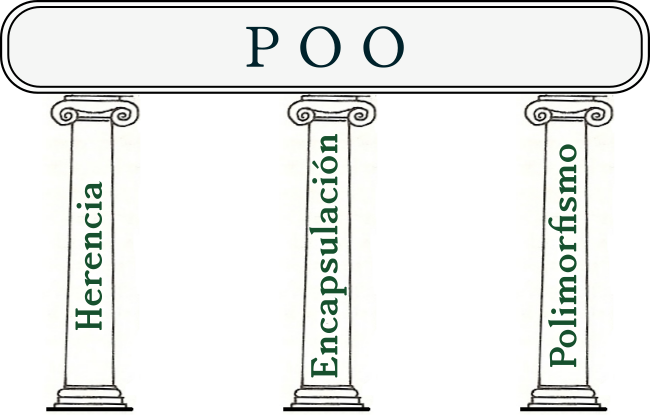
\includegraphics[width=0.4\textwidth]{img/pilares_1.png}
      \caption{Pilares en los que se fundamenta la Programación Orientada a Objetos}
      \label{fig_pilares_1}
   \end{center}
\end{figure}

En relación con el primero de estos pilares, la herencia, es cierto que funciona bien en las típicas jerarquías de clases sencillas que se ponen como ejemplo en los cursos básicos de programación. Es el caso de la clásica descomposición de clases que se muestra en la Figura \ref{fig_figuras}.

\vspace{0.7em}
\begin{figure}[htb]
   \begin{center}
      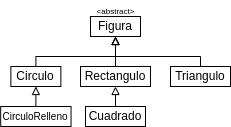
\includegraphics[width=0.5\textwidth]{img/figuras.png}
      \caption{Descomposición típica de clases usada en los cursos de iniciación a la programación}
      \label{fig_figuras}
   \end{center}
\end{figure}
 

El mundo real no siempre se puede modelizar bien haciendo una descomposición en categorías con propiedades bien definidas. Por ejemplo, se puede organizar una jerarquía para el reino animal que divida los animales en mamíferos, reptiles, aves, etc. Y cuando ya está organizada la jerarquía, aparece el ornitorrinco, que no encaja correctamente en ninguna de las categorías que se habían previsto\footnote{\textit{``The platypus effect'' (el efecto ornitorrinco)} es un término acuñado por Anselm Hook y del que yo he tenido conocimiento a través del artículo ``\textit{The Rise and Fall of Object Oriented Programming}'' de David ``Talin'' Joiner.}. La solución puede ser crear una nueva categoría para el ornitorrinco o rehacer la jerarquía de clases para darle cabida. Cualquiera de las dos soluciones es muy costosa en términos de esfuerzo y complejidad.

Es frecuente que las jerarquías de clases sean muy profundas, con muchos niveles de clases que van heredando unas de otras. Las clases en lo alto de la jerarquía tienen métodos y propiedades que solo utilizan unas pocas clases, así como métodos para mantener estados que en muy rara ocasión se modifican. 

A menudo, esta complejidad está originada por tratar de poner juntas cosas que nada tienen en común. Observe la Figura \ref{fig_herencia_composicion}.

\begin{figure}[htb]
   \begin{center}
      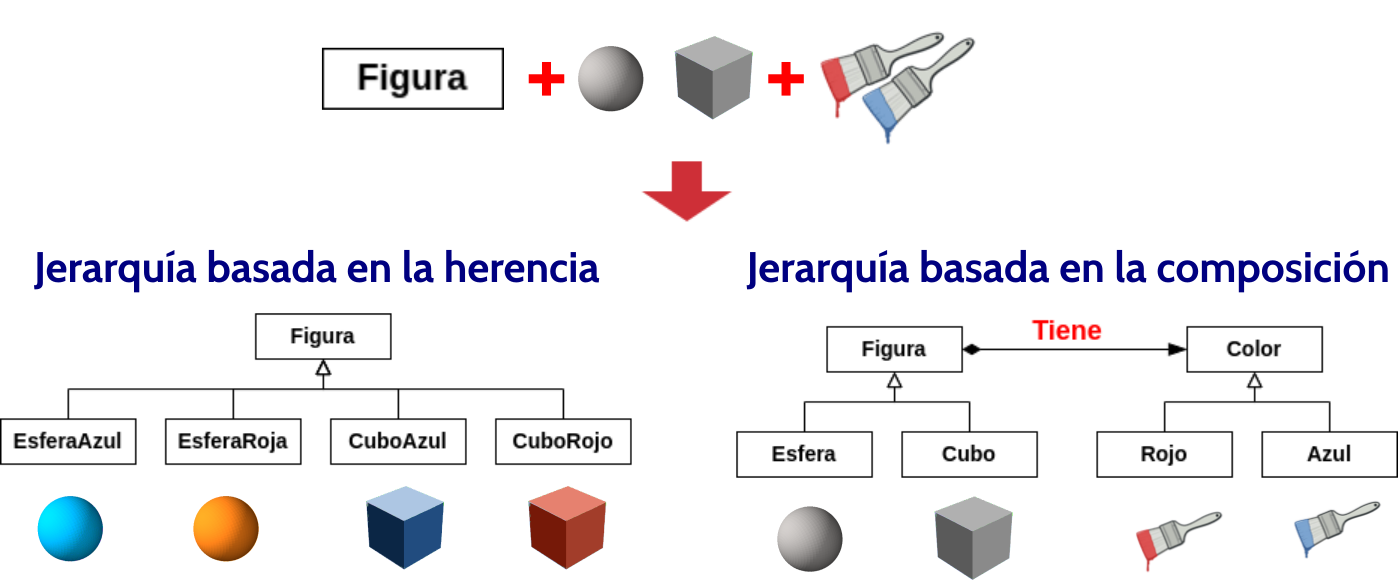
\includegraphics[width=\textwidth]{img/herencia_composicion.png}
      \caption{Diferentes jerarquías de clases según se priorice la herencia o la composición.}
      \label{fig_herencia_composicion}
   \end{center}
\end{figure}

Si se están modelizando figuras, se tienen figuras como la esfera o el cubo. Pero si además se quiere dar cabida a esferas rojas o azules, cubos rojos o azules, etc, se podría caer en crear categorías específicas para las esferas rojas, las esferas azules, los cubos rojos y los cubos azules. Erich Gamma et al., la \textit{banda de los cuatro} (\textit{the Gang Of Four, GoF}), ya indicaron en 1994 en su libro ``Design Patterns''  \citep{gammaDesignPatternsElements1994}, que había favorecer la composición frente a la herencia. En la parte izquierda de la Figura \ref{fig_herencia_composicion} se puede ver la jerarquía de clases que se obtendría priorizando el mecanismo de herencia. En la parte derecha de la misma figura se puede ver el resultado cuando se aplica la composición. 

Otro problema clásico asociado a la creación de jerarquías de clases es el llamado \textit{problema del diamante}, que se esquematiza en la Figura \ref{fig_diamante}. Los lenguajes no suelen permitir que una misma clase herede de dos clases antecesoras, por los problemas que pueden surgir para identificar que método concreto hay que aplicar en determinadas situaciones: ¿qué método \textit{activar()} hereda la \textit{Fotocopiadora}, el del \textit{Scanner} o el de la \textit{Impresora}? La solución, una vez más, es la composición: que la clase \textit{Fotocopiadora} \textit{tenga} una \textit{Impresora} y un \textit{Scanner}, no que derive de ellos. De esta forma, podrá decidir qué método \textit{activar()} utilizará o, quizás, utilizar los dos, uno tras otro.

\vspace{0.7em}
\begin{figure}[htb]
   \begin{center}
      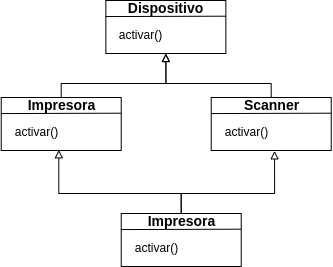
\includegraphics[width=0.5\textwidth]{img/diamante.png}
      \caption{Problema del diamante en una jerarquía de clases}
      \label{fig_diamante}
   \end{center}
\end{figure}

En general, la composición da lugar a jerarquías de clases menos intrincadas, más sencillas de comprender y que se adaptan mejor a las pruebas, la depuración y las modificaciones.

Un problema que no es menor en la POO es que, a medida que las jerarquías de clases crecen, se hace cada vez más difícil preparar test que permitan probar los nuevos métodos que se implementan. Cada nuevo método necesita mucho trabajo de preparación para los test, y esta complejidad se incrementa de manera exponencial a medida que crece la jerarquía de clases.

Modelar el mundo a base de clases y objetos no deja de ser un tema subjetivo: cada programador puede encontrar diferentes formas de entender las categorías necesarias. De hecho, cada entidad de la vida real (clase) puede servir para cosas muy diferentes (métodos de la clase). Una taza puede servir para \textit{beber()}, pero también podría servir como arma para \textit{lanzar()} o como \textit{pisapapeles()}.

Un planteamiento alternativo es que las clases prácticamente solo tengan datos y que las funciones que se necesiten para operar sobre esos datos sean externas a las clases. Esta técnica da lugar a una organización del código mucho más sencilla. Cada función solo realiza una tarea y cuando se quieren hacer test, solo hay que crear algunos juegos de datos de prueba y probar la función concreta, sin tener que luchar con una gran colección de clases y ficheros. Un caso típico donde este planteamiento es muy útil es cuando se trabaja con bases de datos relacionales, que se adaptan mal a la modelización de la POO.


Una de las \textit{promesas} que se asociaba al paradigma de la POO es la reutilización. Suponga que tiene que desarrollar una aplicación y que ya dispone de una jerarquía de clases que se ha utilizado en una aplicación anterior. Surge la necesidad en la nueva aplicación de utilizar una clase similar a una que ya se utilizó en la aplicación anterior y se opta por copiar  y pegar la clase en la nueva aplicación. Pero el programa no compila; dicha clase deriva de otra y esa otra de otra... Al final, es necesario trasladar a la nueva aplicación la clase que se necesita y toda la jerarquía de clases de las que hereda, que pueden no tener ninguna utilidad en la nueva aplicación. Pero sigue sin compilar; resulta que alguna de las clases de esa jerarquía utiliza otra clase que a su vez tiene su propia jerarquía. Al final, para reutilizar una clase concreta, hay que trasladar a la nueva aplicación un montón de clases que no se necesitan en absoluto... o hacer la clase nueva y olvidarse de reutilizar. Joe Armstrong, el creador del lenguaje Erlang, denominaba a este problema el \textit{problema del gorila}: necesito un plátano y termino trayéndome el gorila que sostiene el plátano y, con él, toda su selva\footnote{Esta cita de Armstrong y algunas de las ideas y ejemplos que se muestran en este apartado proceden de artículos escritos por Charles Scalfani, autor del libro ``\textit{Functional Programming Made Easier}'' \citep{scalfaniFunctionalProgrammingMade2021}.}.

Hay problemas más sutiles asociados con la reutilización de clases. Observe el código Java siguiente:

\vspace{0.7em}
\begin{Codigo}
class Array {
   private ArrayList<Object> a = new ArrayList<Object>();
   
   public void add(Object element) {
      a.add(element);
   }
   public void addAll(Object elements[]) {
      for (int i = 0; i < elements.length; ++i)
      a.add(elements[i]); // Esta línea va a cambiar
   }
}
\end{Codigo}

 Se trata de una clase llamada \textit{Array} que proporciona un método \textit{add()}, para añadir elementos individuales y un método \textit{addAll()}, que permite añadir un array ordinario de objetos en una sola operación. 
 
 Suponga ahora que, en nuestra aplicación, derivamos una clase llamada \textit{ArrayCount}, que añade un contador a la clase \textit{Array}. Nuestra clase sobreescribe los métodos de la clase base para gestionar el valor del contador. El código podría ser el siguiente:
  
\vspace{0.7em}
\begin{Codigo}
public class ArrayCount extends Array {
   private int count = 0;

   @Override
   public void add(Object element) {
      super.add(element);
      ++count;
   }
\end{Codigo}

\begin{Codigo}
   @Override
   public void addAll(Object elements[]) {
      super.addAll(elements);
      count += elements.length;
   }
   public int getCount() {
      return this.count;
   }
}
\end{Codigo}

El código para probar nuestra clase \textit{ArrayCount} podría ser el siguiente:

\vspace{0.7em}
\begin{Codigo}
public class Main {
   
   public static void main(String[] args) {
      Integer[] list = {1, 2, 3};
      ArrayCount ac = new ArrayCount();
      ac.addAll(list);
      System.out.println(ac.getCount()); // Imprime 3
   }
}
\end{Codigo}

Si se ejecuta, el programa mostrará que el contador de elementos vale 3, que es el valor correcto.

La clase original podría ser el código de una librería y que solo pudiéramos utilizar los métodos que proporciona, sin que tuviéramos acceso al código fuente. Suponga que los creadores de la librería realizan un cambio en la clase base. El cambio solo afecta al método \textit{addAll()}: en lugar de actuar directamente sobre el \textit{ArrayList}, llaman a su propio método \textit{add()}, como muestra el siguiente código:

\vspace{0.7em}
\begin{Codigo}
public void addAll(Object elements[]) {
   for (int i = 0; i < elements.length; ++i) {
      add(elements[i]); // Esta línea ha cambiado
   }
}
\end{Codigo}

Aparentemente el cambio es inocuo. Los creadores de la librería comprueban que la nueva función pasa todos los test y que el cambio no afecta en nada a la funcionalidad de la librería. Pero nuestro programa falla: si ejecutamos el programa, el contador muestra 6, en lugar de 3. No podemos saber qué está pasando, pues no tenemos acceso al código fuente y nos es imposible saber cuál es el problema.

Este tipo de problemas podría llevarnos a la conclusión de que nunca hay que derivar una clase de otra de la que no tengamos acceso al código fuente.

Hay más problemas asociados a la creación de las jerarquías de clases. Las jerarquías de clases están pensadas para que las clases derivadas sean especializaciones de las clases antecesoras. El planteamiento es que las jerarquías se basen en \textit{categorizar} las clases derivadas. Pero en el mundo real no se suelen encontrar jerarquías de ese tipo, es más frecuente encontrar jerarquías en las que unas clases de objetos contienen a otros. En esos casos, la jerarquía de herencia que ofrecen los lenguajes de programación no se adaptan bien a la modelización de dichas jerarquías. Piense en el caso de una base de datos relacional, con sus tablas, sus registros, sus columnas, sus índices, sus relaciones entre las distintas tablas, etc. No está claro que clases derivan de otras, es más fácil pensar en términos de que unas clases \textit{contienen} a otras. En esos casos, la herencia es de poca ayuda. Hay otros casos con problemas similares, por ejemplo la estructura de ficheros y directorios de un sistema de archivos, o muchas otras.
  
El segundo pilar en el que se apoya la POO es la encapsulación. 
Una de las reglas que se considera que debe cumplir cualquier diseño orientado a objetos es la \textit{encapsulación}, según la cual, el estado de los objetos no se debe poder modificar directamente desde fuera del objeto, sino solo a través de los métodos que proporciona la clase en cuestión. 

Por ejemplo, si se tuviera una clase denominada \textit{Etiqueta} con una propiedad llamada \textit{texto}, no se debería poder borrar el texto de la etiqueta mediante una instrucción del tipo:

{\centering \texttt{etiqueta.text = `` '';} \par}

Un diseño correcto proporcionaría un método \textit{borrar()} que realizase dicha acción de borrar el texto de la etiqueta:

{\centering \texttt{etiqueta.borrar();} \par}

Este procedimiento funciona perfectamente cuando las operaciones son sencillas, pero la cosa se complica cuando las acciones a realizar implican varios objetos de distintas clases. En esos casos, puede ser más sencillo utilizar funciones ajenas a las propias clases. Es una cuestión casi semántica: ¿en qué debemos poner más énfasis, en los sustantivos (\textit{Etiqueta}) o en los verbos (borrar()).

La encapsulación parece proteger los datos internos de la clase de su acceso desde el exterior. Pero resulta que la mayoría de los lenguajes, cuando pasan un objeto a una función, lo que pasan no es una copia del objeto original, sino una referencia al mismo. Esto se hace por motivos de eficiencia. 

Suponga el constructor de una clase recibe una referencia a un objeto que guarda en una propiedad privada interna. Por ejemplo, la clase \textit{Circulo} recibe en su constructor un \textit{Punto} que hace las veces de centro del círculo. Si lo que recibe \textit{Circulo} es una referencia a un \textit{Punto}, el programa que está instanciando la clase tiene acceso a dicha referencia y podría modificar las coordenadas del punto sin utilizar los métodos de \textit{Circulo}. 

Una forma de resolver este problema es no pasar nunca referencias a objetos, pasar copias de los objetos. Hay que crear clones de los objetos realizados como \textit{deep copies}, esto es, hay que copiar recursivamente todos los niveles del objeto que se quiere clonar. En el caso del \textit{Circulo}, en vez de pasar un \textit{Punto} en el constructor, podríamos pasar directamente las coordenadas \textit{x} e \textit{y} del centro. Lo habitual es que los lenguajes, cuando pasan un tipo primitivo como argumento a una función, pasen una copia del valor, no una referencia al mismo. 

Pero no todos los objetos se pueden copiar. En los programas se usan referencias a componentes del sistema operativo como los manejadores de ficheros que no se pueden clonar, o \textit{sockets} de una conexión u otros elementos que no admiten ser clonados. En esos casos, la propiedad interna del objeto estaría siempre expuesta a su acceso desde el exterior, rompiendo la regla de la encapsulación.
 
El tercer pilar en el que se basa la POO es el polimorfismo. No es que el polimorfismo no sea bueno, es que para disponer de él no es necesario un lenguaje orientado a objetos, es suficiente con implementar el polimorfismo basado en la herencia de interfaces. 

Esta última, es la solución que ha implantado Rust. En Rust, los objetos se modelizan con los tipos \textit{struct} o \textit{enum}. Como se verá en el Apartado \ref{sec_tipos_personalizados}, los tipos \textit{struct} y \textit{enum} tienen datos y métodos, pero no disponen de un mecanismo de herencia entre tipos. En Rust, el tipo \textit{trait} sería el equivalente a los interfaces de otros lenguajes. Los \textit{traits} sí tienen la posibilidad de implementar el mecanismo de herencia. También se puede imponer que cualquier tipo de datos \textit{implemente} uno o más \textit{traits}. Con ello y con los denominados \textit{tipos genericos}, se dispone de todos los elementos necesarios para utilizar un polimorfismo más flexible y con menos acoplamientos que el que resulta del polimorfismo basado en la herencia entre objetos. En el Apartado \ref{sec_traits} se explicará cómo hacerlo.

En Java también es posible utilizar los interfaces y la herencia entre interfaces para conseguir este tipo de polimorfismo. De hecho, priorizando este mecanismo y la composición, en vez de la herencia, se consiguen códigos más flexibles y desacoplados que siguiendo el método tradicional jerarquías basadas en la herencia.

\vspace{0.7em}
\begin{figure}[htb]
   \begin{center}
      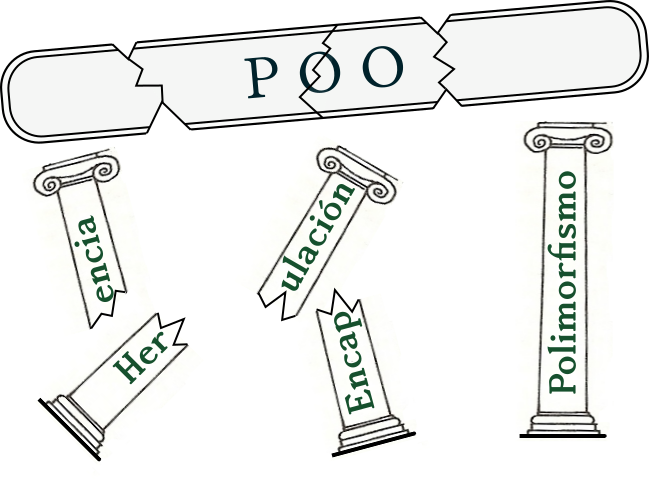
\includegraphics[width=0.5\textwidth]{img/pilares_2.png}
      \caption{No es necesaria la POO para disponer de polimorfismo}
      \label{fig_pilares_2}
   \end{center}
\end{figure}

\section{¿En qué consiste la programación funcional?}
\noindent Es difícil definir el concepto de \textit{Programación Funcional} (PF). Se considera que la PF está incluida en el paradigma de la \textit{programación declarativa}, en la cual los lenguajes se centran en describir qué quieren hacer en lugar de detallar cómo hacerlo, como sucede en los lenguajes imperativos.

Los siguientes elementos formarían parte del conjunto de componentes que utilizan los lenguajes funcionales:

\begin{itemize}
   \item \textbf{Funciones puras:} se dice que una función es \textit{pura} si no produce efectos secundarios, no depende de ningún estado exterior y siempre proporciona el mismo resultado para el mismo valor de los argumentos de entrada. Se entiende por \textit{efecto secundario} cualquier acción de la función que afecte a algo fuera del contexto de la propia función. Por ejemplo, modificar el estado de una variable global, mostrar un mensaje en una pantalla o enviar un correo electrónico serían ejemplos de efectos secundarios.
   
   \vspace{1em}
   
   \item \textbf{Funciones de orden superior:} las funciones que operan utilizando otras funciones se denominan \textit{funciones de orden superior}. En la programación funcional, las funciones se consideran \textit{elementos de primera clase}, lo que significa que se pueden tratar como cualquier otro tipo de datos: se pueden utilizar como parámetros o como valor devuelto por otras funciones y pueden asignarse a variables. En la mayoría de lenguajes hay elementos que no son de primera clase, por ejemplo los operadores o las cláusulas que definen los bucles o las bifurcaciones.
   
   \vspace{0.5em}

   \item \textbf{Closures:} en programación funcional es habitual utilizar un tipo especial de funciones denominadas \textit{closures}. Se trata de funciones anónimas definidas in situ que son capaces de capturar el entorno en el que fueron definidas, de forma que pueden acceder con posterioridad a variables de ese entorno con los valores que tuvieran en el momento en el que se declaró la \textit{closure}. Actualmente, las \textit{closures} también se incluyen en numerosos lenguajes, a veces bajo la denominación de \textit{funciones anónimas}.
   
   \vspace{0.5em}

   \item \textbf{Inmutabilidad:} la programación funcional pone especial énfasis en la utilización de estructuras \textit{inmutables}. Cambiar el valor de una variable, cambiar su estado, se considera un efecto secundario que hay que tratar de evitar. Decir que las \textit{variables} no deben variar puede parecer un contrasentido, pero no es excepcional en los lenguajes de programación. Por ejemplo, en Java o en Javascript, las variables del tipo \textit{String} son inmutables. Cuando se quiere modificar el estado de una variable inmutable lo que se hace es crear una nueva variable con el nuevo valor. El procedimiento consiste en \textit{transformar} una variable en otra, en vez de en modificar el estado de la variable original. La inmutabilidad facilita los test de los programas y hace más segura la utilización de la programación multiproceso o en paralelo.
   
   \vspace{0.5em}

   \item \textbf{Recursividad:} el control de flujo en la programación funcional favorece la recursividad frente a los bucles. Sustituyendo los bucles del tipo \textit{for} o \textit{while} mediante recursividad se consigue un código más declarativo y, en ocasiones, más elegante.
   
   \vspace{0.5em}

   \item \textbf{Iteradores:} los \textit{iteradores} son una construcción habitual en la programación funcional y que, a día de hoy, incorporan muchos lenguajes. Son estructuras que permiten recorrer una colección de manera ordenada, sin recurrir a bucles y variables de índice. 
   
   \vspace{0.5em}

   \item \textbf{Evaluación perezosa:} las expresiones, siempre que se pueda, se deben comportar de manera \textit{perezosa}. La \textit{evaluación perezosa} (\textit{lazy evaluation}) consiste en que determinados cálculos que impliquen a variables no se realicen hasta que son estrictamente necesarios.
   
   \vspace{0.5em}

   \item \textbf{Sin estado ni efectos secundarios:} en la programación funcional se trata de minimizar los estados mutables y los efectos secundarios. El resultado es un código en el que es más fácil razonar, hacer test y realizar la depuración de errores. Cuando es necesario mantener estados o realizar acciones con efectos secundarios, se controla rigurosamente.
\end{itemize}

Tras leer los párrafos anteriores, el lector puede estar preguntándose cómo es posible realizar un programa de aplicación práctica sin efectos secundarios y sin cambiar el valor de las variables. Bien, no es posible, los programadores funcionales utilizan funciones impuras en numerosas ocasiones y necesitan utilizar variables mutables en determinados contextos. No obstante, durante el desarrollo de un programa, hay numerosas situaciones en las que la utilización de funciones puras y el respeto a la inmutabilidad proporciona más seguridad y da lugar a que el código generado sea más escalable.

La programación funcional no es una sintaxis determinada, consiste en una serie de técnicas orientadas a eliminar los efectos secundarios o, al menos, limitar su alcance. Si se utilizan estas técnicas de manera adecuada, se consigue escribir código más fácil de leer, más correcto, más seguro, más fácil de probar y más fácil de depurar, lo que a fin de cuentas es el objetivo fundamental que se debe perseguir al programar. 

La técnicas de la programación funcional no están restringidas por el lenguaje de programación que se utilice. Los conceptos que se utilizan en la programación funcional se pueden aplicar a la programación orientada a objetos o a la programación basada en procedimientos. Son principios generales que producen beneficios en la codificación de cualquier programa y en cualquier lenguaje. En realidad se trata de buenas prácticas de codificación de carácter universal.

\section{Diferencias con la Programación Orientada a Objetos}
\noindent Mientras que la Programación Orientada a Objetos se centra en la interacción y la comunicación entre diferentes objetos, la Programación Funcional se centra en cómo se van transformando los objetos. Dicha transformación hay que entenderla en el sentido de que un objeto se le pasa como argumento a una función que devuelve un nuevo objeto que incorpora las transformación que se quiere realizar. El objeto que devuelve la función es un nuevo objeto y el objeto original se puede conservar o desechar. En la Programación Funcional, unos objetos se transforman en otros, no se modifican.

\vspace{2em}
   
Se resumen a continuación algunas de las características de la programación orientada a objetos (POO):
\begin{itemize}
   \item \textbf{Estado de los objetos:} la POO está basada en objetos que encapsulan en una sola entidad su estado (propiedades) y su comportamiento (métodos). La \textit{mutabilidad} es una parte inherente de la POO. El estado de los objetos puede variar a lo largo del tiempo, lo que se consigue a través de los métodos que proporcionan las clases. De esta manera, se modelizan las entidades reales y sus relaciones. Esta mutabilidad es una forma natural de representar las propiedades de los objetos que necesitan cambiar de valor a lo largo del tiempo, pero da lugar a problemas complejos para gestionar estados globales y secundarios, por ejemplo en la programación concurrente.

   \vspace{0.5em}

   \item \textbf{Clases y herencia entre tipos:} la POO se basa en el concepto de clases como modelos de los objetos y a menudo utiliza la herencia entre clases para compartir y ampliar el comportamiento de las mismas.

   \vspace{0.5em}
   
   \item \textbf{Polimorfismo:} objetos de diferentes clases pueden ser tratados como si fueran de una misma clase base de la cual todos derivan.
   
   \vspace{0.5em}
      
   \item \textbf{Paradigma imperativo:} en general, la POO utiliza código con un paradigma imperativo, describiendo los pasos que hay que dar para modificar el estado de los objetos.
\end{itemize}

En el caso de la programación funcional (PF), algunas características distintivas son:
\begin{itemize}
   \item \textbf{Funciones sin estado:} está basada en la utilización de funciones que no mantienen ningún estado y operan sobre datos inmutables. En ese sentido, la PF separa el estado de los objetos de su comportamiento. El estado se representa mediante estructuras de datos inmutables. El comportamiento se expresa a través de funciones que operan sobre dichos datos.
   
   \vspace{0.5em}
   
   \item \textbf{Funciones como objetos de primera clase:} las funciones son objetos de primera clase que se pueden utilizar como parámetros de otras funciones, se pueden devolver como resultados y se pueden asignar a variables. Las funciones se utilizan para modelizar abstracciones, encapsular comportamientos. Para conseguir procesamientos complejos se utiliza la composición de funciones.
   
   \vspace{0.5em}

   \item \textbf{Paradigma declarativo:} la PF utiliza una codificación más declarativa, expresando la lógica de lo qué se quiere hacer, sin describir el flujo de instrucciones para ello. 
\end{itemize}

La opinión del autor es que no hay que ser fundamentalista de ningún paradigma de programación. Hay que recordar el viejo dicho: ``\textit{al que la única herramienta que conoce es el martillo, todo le parecen clavos}''. Hay problemas que se adaptan mejor a unas técnicas de programación u otras. En muchas ocasiones, una combinación adecuada de las técnicas de la POO y de la PF será lo más adecuado. En todos los casos hay que analizar el problema que se trata de resolver y utilizar la combinación de técnicas que mejor se adapte al mismo.

